\documentclass[pmlr,twocolumn,10pt]{jmlr}
% ML4H 2026 proceedings track (anonymous review). NOTE: the official ML4H
% Overleaf template defines \mlhtrack and \finalfalse/\finaltrue; stubbed here
% so this compiles with vanilla jmlr.cls. Move content into the official
% template before submitting.
\providecommand{\mlhtrack}[1]{}
\mlhtrack{proceedings}
\usepackage{tikz}
\usetikzlibrary{arrows.meta,positioning,fit,backgrounds,calc}
\usepackage{pgfplots}\pgfplotsset{compat=1.16}
\usepackage{xcolor}
\usepackage{calc}
\usepackage{booktabs}
\usepackage{graphicx}
\usepackage{adjustbox}
\usepackage{placeins}
\usepackage{microtype}
% ---- colour palette ----
\definecolor{cblue}{HTML}{3A6EA5}
\definecolor{caccent}{HTML}{0F6E5C}
\definecolor{cclay}{HTML}{BD5B36}
\definecolor{cpaper}{HTML}{F3F5F3}
\definecolor{cline}{HTML}{C5CDC8}
\definecolor{cmuted}{HTML}{5C6B64}
\definecolor{ckhaki}{HTML}{7A6A3A}
\definecolor{hgreen}{HTML}{CDEBD9}
\definecolor{hyellow}{HTML}{F6E7A6}
\definecolor{hred}{HTML}{F3C9C4}
\newcommand{\oldv}[1]{\textcolor{cclay}{#1}}
\newcommand{\newv}[1]{\textcolor{caccent}{\textbf{#1}}}
\setlength{\fboxsep}{1pt}
\newcommand{\hg}[1]{\colorbox{hgreen}{#1}}
\newcommand{\hy}[1]{\colorbox{hyellow}{#1}}
\newcommand{\hr}[1]{\colorbox{hred}{#1}}
\newcommand{\card}[1]{\begin{center}\fcolorbox{cline}{cpaper}{\parbox{0.94\linewidth}{\small #1}}\end{center}}
\newcommand{\arr}{\,$\rightarrow$\,\allowbreak}
\newcommand{\tp}[1]{\texttt{#1}}
\newcommand{\pending}[1]{\textcolor{red}{#1}}
\newcommand{\nk}[1]{{\footnotesize\textcolor{ckhaki}{#1}}}
\newcommand{\vc}[2]{#1\,{\scriptsize\textcolor{ckhaki}{$\pm$#2}}}
\setlength{\tabcolsep}{4pt}
\sloppy \setlength{\emergencystretch}{3em}

\jmlrworkshop{Machine Learning for Health (ML4H) 2026}
\jmlryear{2026}
\jmlrvolume{XXX}
\jmlrpages{XX}
\editor{Editors: to be assigned}
\title[Surrogate Substitution Preserves PHI Detectability]{Surrogate Substitution Preserves PHI Detectability:\\ A Multi-Detector Equivalence Study}
\author{\Name{Anonymous Author(s)}}

\begin{document}
\maketitle

\begin{abstract}
Structure-preserving de-identification replaces protected health information (PHI) with realistic same-type \emph{surrogates}---``Anna~S.'' becomes ``Maria~S.'', not \tp{[NAME]}---so that clinical text stays fluent and downstream tools keep working. But this only helps if the substitution does not itself corrupt the signal those tools rely on. We ask a narrow, testable question: \emph{on the spans a de-identifier actually masks, can downstream PHI detectors still find the surrogate?} We introduce a paired, multi-detector evaluation protocol that (i)~scores utility \emph{only on masked spans}, decoupling \emph{coverage} from \emph{utility}; (ii)~uses \emph{equivalence testing} (TOST) rather than null-hypothesis significance testing, which is uninformative at our sample size (57k paired spans); and (iii)~builds a surrogate-failure typology separating fixable generator defects from intrinsic detector limits. Across 11 detectors, 7 benchmarks, and 7 languages (1{,}750 documents), recall on masked spans moves from 76.1\% to 74.9\%---a change our equivalence test shows is \emph{statistically equivalent to zero within a $\pm2$-point margin} ($p\approx3\times10^{-9}$), with detector ranking preserved. The residual loss does not reflect detectors getting worse at PHI: it concentrates in \emph{malformed and out-of-distribution} surrogates (truncation \tp{Chicago}\arr\tp{Illino}, salience loss \tp{Cedars-Sinai}\arr\tp{Vidant}). A redaction floor and an open-source surrogate baseline, run across detector families, indicate the effect is a property of well-formed substitution---not of one tool or one detector. We release the evaluation subsets, scoring code, and an interactive dashboard (URLs withheld for anonymous review) so the protocol can audit any structure-preserving transform.
\end{abstract}

\section{Introduction}
De-identification of clinical text takes two forms---and only one keeps the text usable downstream. \textbf{Redaction} deletes or tags PHI (\oldv{\tp{John Smith}}~$\rightarrow$~\tp{[NAME]}), which is safe but destroys the fluency, layout, and distributional properties that downstream models and human readers depend on. \textbf{Structure-preserving} de-identification instead substitutes each PHI value with a plausible, same-type \emph{surrogate} (\oldv{\tp{John Smith}}\arr\newv{\tp{Maria Lopez}}), keeping the document readable and machine-parseable~\citep{carrell2013hiding}. The second family is increasingly attractive: it lets de-identified data flow into analytics, model training, and even second-pass detection without breaking pipelines built for real text.

The promise of structure preservation rests on an unstated assumption: \emph{the surrogate carries the same downstream signal as the value it replaced.} If substitution silently degrades the very features a PHI detector, an NER model, or a clinical parser relies on, then ``structure-preserving'' is a misnomer---the transform would be quietly laundering PHI into forms tools can no longer see or handle, which is both a utility problem and, for a second-pass safety net, a privacy problem.

This assumption is rarely tested directly, and testing it well is harder than it looks. Three pitfalls recur:
\begin{enumerate}\itemsep2pt
\item \textbf{Coverage confounds utility.} A de-identifier that masks 60\% of PHI and one that masks 95\% cannot be compared on whole-document F1---the score conflates \emph{how much} it masks with \emph{whether what it masks stays usable}. The two must be measured separately.
\item \textbf{The large-$N$ significance trap.} With tens of thousands of paired spans, any non-zero difference is ``statistically significant'' under a standard test, even when operationally meaningless. A $p$-value here answers the wrong question.
\item \textbf{Aggregate error hides mechanism.} A single ``$-1.2$ points'' says nothing about \emph{why} the loss happens---boundary jitter, detector weakness, or a defect in surrogate generation. Only the last is fixable, and only an error typology tells them apart.
\end{enumerate}

We address all three. Our contributions:
\begin{itemize}\itemsep2pt
\item A \textbf{paired multi-detector protocol} scoring utility on masked spans only, decoupling coverage from utility, across 11 detectors $\times$ 7 benchmarks $\times$ 7 languages (\S\ref{sec:protocol}--\S\ref{sec:design}).
\item An \textbf{equivalence-testing analysis} (TOST) replacing the uninformative significance test with a bounded-effect claim: the change in detectability is bounded within $\pm2$ points of zero (\S\ref{sec:results}).
\item A \textbf{surrogate-failure typology} attributing the small residual to surrogate-generation quality rather than detectors getting worse at PHI (\S\ref{sec:error}).
\item A set of \textbf{comparison experiments}---a redaction upper-bound and an open-source surrogate baseline---that make the result reproducible and isolate what is generic to \emph{any} substitution versus specific to one tool (\S\ref{sec:design},~\S\ref{sec:results}).
\end{itemize}
The framing is deliberately not ``a proprietary tool is good.'' It is: \emph{here is how to measure whether a structure-preserving transform preserves utility, rigorously}, with one commercial transform as the case study and open baselines for reproducibility.

\section{Related Work}
\subsection{De-identification and surrogate substitution}
Clinical de-identification is a long-studied sequence-labeling problem~\citep{uzuner2007evaluating}, anchored by the i2b2/n2c2 and MEDDOCAN shared tasks~\citep{stubbs2015i2b2,marimon2019meddocan} and by systems ranging from rule- and dictionary-based pipelines~\citep{presidio} through recurrent and transformer taggers~\citep{dernoncourt2017deid,liu2017deid,johnson2020deid} to instruction-tuned LLMs used zero-shot~\citep{liu2023deidgpt}. Most of this literature optimizes \emph{detection}, typically against the HIPAA Safe Harbor identifier set~\citep{hhs2012safeharbor}. The downstream question---\emph{what to put in the PHI's place}---is comparatively under-studied. Surrogate (``hiding in plain sight'') replacement was proposed to keep de-identified notes realistic and to resist re-identification~\citep{carrell2013hiding}; subsequent work showed poor surrogates can even aid re-identification (the ``parrot'' attack), underscoring that surrogate \emph{quality} matters~\citep{carrell2020parrot}. Recent studies generate surrogates or synthetic notes with rule-based and LLM methods and measure the downstream trade-off~\citep{yermilov2023privacy,kim2024generalizing}, while a parallel line shows de-identified or pseudonymized text can still leak under extraction and membership-inference attacks~\citep{carlini2021extracting,lehman2021bert,sarkar2024deid}---so a surrogate must both \emph{destroy} the original (privacy) and \emph{remain a well-formed, same-type value} (utility). Our work is orthogonal to the detection literature and to any particular surrogate generator: given that a span is masked, we ask whether the \emph{replacement} remains detectable and well-formed.

The commercial transform used as our case study is a proprietary, structure-preserving de-identification API (vendor and product name withheld for anonymous review); we treat it as the source of the transform rather than describing or extending the method.

\subsection{Utility-preservation evaluation}
Whether privacy transformations preserve downstream utility is central to privacy-preserving NLP. \citet{vakili2022downstream} find automatic de-identification---including realistic surrogate replacement---barely affects downstream clinical model quality, and \citet{vakili2023mia} caution that the measurement instrument matters. Prior evaluations typically run a single downstream model on original vs.\ transformed data and compare end-task scores. Two weaknesses recur: (a)~a single downstream model cannot separate ``the transform is fine'' from ``this model is robust,'' and (b)~whole-corpus metrics mix masked and unmasked content. We address (a)~with an 11-detector panel spanning rule-based, fine-tuned, and LLM detectors, and (b)~by restricting utility measurement to masked spans.

\subsection{The large-$N$ trap and equivalence testing}
When samples are large, null-hypothesis significance testing rejects the null for negligible effects; the $p$-value measures precision, not importance---a hazard increasingly flagged in NLP evaluation~\citep{dror2018hitchhiker,card2020power}. The standard remedy is \emph{equivalence testing}---the two one-sided tests (TOST) procedure~\citep{schuirmann1987tost,berger1996bioequivalence}---which specifies an equivalence margin $\Delta$ and tests whether the effect lies inside $[-\Delta,+\Delta]$; see \citet{lakens2017tost,lakens2018equivalence} for practical tutorials. TOST is standard in biostatistics but under-used in NLP evaluation, where large paired corpora make the trap acute. We adopt it as the primary inferential tool and report McNemar's paired test~\citep{mcnemar1947} only to demonstrate the trap.

\section{Problem Formulation}
\textbf{Structure-preserving de-identification.} A transform $T$ maps a document $d$ to $d'$ by replacing each detected PHI value $v$ (of type $\tau$) with a surrogate $s$ of the same type, leaving all other characters unchanged. Gold PHI spans on $d$ are re-projected onto $d'$ by character-level alignment, giving paired spans $(v,s)$.

\textbf{Coverage vs.\ utility.} Two quantities must not be conflated. \emph{Coverage} is the fraction of true PHI that $T$ detects and replaces (a property of $T$'s detector). \emph{Utility} is, given that a span was replaced, whether a downstream detector still finds the surrogate $s$ as well as it found $v$ (a property of $T$'s generator and of the surrogate's realism). We report coverage separately and measure utility \emph{only on the masked-span population} $\{(v,s)\}$. This prevents a low-coverage transform from looking good---or a high-coverage one from looking bad---on a metric that is really about substitution quality.

\begin{figure*}[t]
\centering
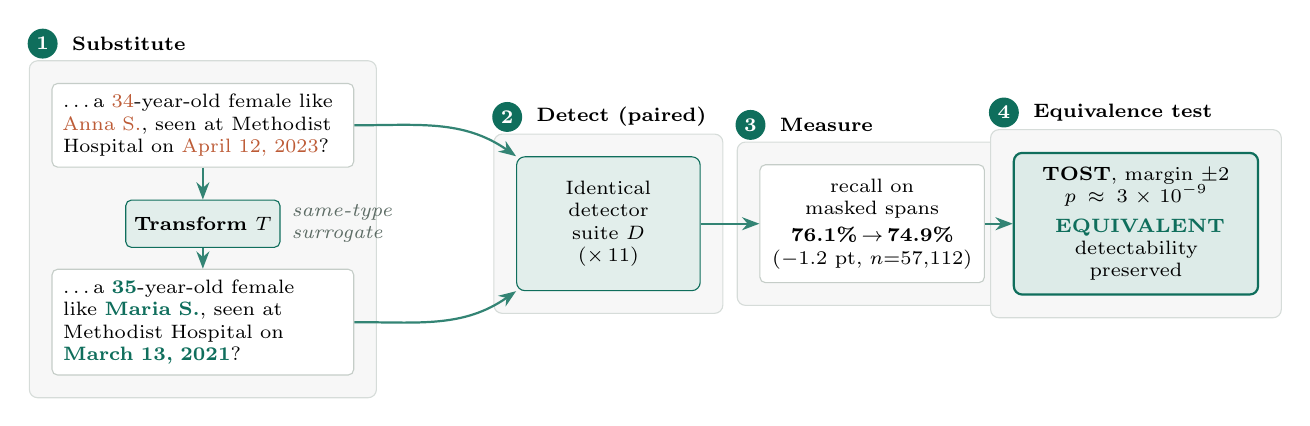
\begin{tikzpicture}[font=\scriptsize,>={Stealth[length=2.2mm]},
  card/.style={draw=cline,fill=white,rounded corners=2pt,inner sep=4pt,align=left,text width=3.55cm},
  op/.style={draw=caccent,fill=caccent!12,rounded corners=2pt,inner sep=3pt,align=center,minimum height=6mm,font=\scriptsize\bfseries},
  det/.style={draw=caccent,fill=caccent!12,rounded corners=3pt,inner sep=4pt,align=center,text width=2.05cm,minimum height=17mm},
  meas/.style={draw=cline,fill=white,rounded corners=2pt,inner sep=5pt,align=center,text width=2.5cm},
  verdict/.style={draw=caccent,line width=0.8pt,fill=caccent!14,rounded corners=3pt,inner sep=5pt,align=center,text width=2.75cm},
  flow/.style={->,thick,caccent!85},
  panel/.style={rounded corners=3pt,fill=black!3,draw=cline!70,inner sep=8pt},
  badge/.style={circle,fill=caccent,text=white,font=\scriptsize\bfseries,inner sep=0.6pt,minimum size=3.8mm}
]
% ---- Stage 1: substitute (with a concrete worked example) ----
\node[card] (co) at (0,1.25) {\dots a \oldv{34}-year-old female like \oldv{Anna S.}, seen at Methodist Hospital on \oldv{April 12, 2023}?};
\node[op]   (T)  at (0,0)    {Transform $T$};
\node[card] (ct) at (0,-1.25){\dots a \newv{35}-year-old female like \newv{Maria S.}, seen at Methodist Hospital on \newv{March 13, 2021}?};
\draw[flow] (co.south) -- (T.north);
\draw[flow] (T.south) -- (ct.north);
\node[font=\scriptsize\itshape,text=cmuted,right=1pt of T,text width=1.5cm] {same-type surrogate};
% ---- Stage 2: detect (paired) ----
\node[det] (det) at (5.15,0) {Identical\\ detector\\ suite $D$\\ ($\times\,11$)};
\draw[flow] (co.east) to[out=0,in=145] (det.north west);
\draw[flow] (ct.east) to[out=0,in=215] (det.south west);
% ---- Stage 3: measure ----
\node[meas] (m) at (8.5,0) {recall on masked spans\\[2pt]\textbf{76.1\%}\,$\rightarrow$\,\textbf{74.9\%}\\{\scriptsize($-1.2$ pt, $n{=}57{,}112$)}};
\draw[flow] (det.east) -- (m.west);
% ---- Stage 4: equivalence test ----
\node[verdict] (v) at (11.85,0) {\textbf{TOST}, margin $\pm2$\\ $p\approx3\times10^{-9}$\\[3pt]{\color{caccent}\textbf{\checkmark\ EQUIVALENT}}\\{\scriptsize detectability preserved}};
\draw[flow] (m.east) -- (v.west);
% ---- background stage panels + numbered titles ----
\begin{scope}[on background layer]
  \node[panel,fit=(co)(ct)(T)] (p1) {};
  \node[panel,fit=(det)] (p2) {};
  \node[panel,fit=(m)] (p3) {};
  \node[panel,fit=(v)] (p4) {};
\end{scope}
\foreach \p/\n/\ttl in {p1/1/Substitute,p2/2/Detect (paired),p3/3/Measure,p4/4/Equivalence test}{
  \node[badge] (b\p) at ([xshift=5pt,yshift=6pt]\p.north west) {\n};
  \node[anchor=west,font=\scriptsize\bfseries,text=black] at (b\p.east) {\,\ttl};
}
\end{tikzpicture}
\caption{\textbf{The paired evaluation protocol, with a worked example.} \textbf{(1)}~The transform replaces each PHI value with a same-type surrogate (\oldv{original}~$\rightarrow$~\newv{surrogate}), leaving everything else byte-identical. \textbf{(2)}~The \emph{identical} 11-detector suite scores \emph{both} the original $d$ and the transformed $d'$, so any per-span change is attributable to the substitution alone. \textbf{(3)}~Utility is measured \emph{only on the spans the transform masks} (overlap match), decoupling it from coverage. \textbf{(4)}~The paired recall difference is assessed with an equivalence test (TOST, margin $\pm2$ pts) rather than a significance test---which the large sample would make trivially ``significant'' (\S\ref{sec:protocol}). Result: the change is statistically equivalent to zero.}
\label{fig:protocol}
\end{figure*}

\section{Evaluation Protocol}\label{sec:protocol}
Figure~\ref{fig:protocol} summarizes the protocol. \textbf{Paired multi-detector design.} Each document is scored in two conditions---original $d$ and transformed $d'$---by the \emph{identical} detector suite $D$ ($|D|=11$). Because the only change between conditions is the substitution, any per-span change in detection is attributable to the substitution, not to the detector or the document.

\textbf{Metrics.} We report span-level P/R/F1 under three matching modes---\emph{exact} (start+end+type), \emph{type} (type+boundary), \emph{overlap} (any character overlap+type)---and \emph{leakage}~$=1-\text{recall}$, the HIPAA-critical quantity. The headline utility metric is \emph{recall retention on masked spans}~$=\text{recall}(d')/\text{recall}(d)$ restricted to $\{(v,s)\}$, under overlap matching (so pure boundary jitter from length changes, ``Anna~S.''$\rightarrow$``Maria~S.'', is not charged as a miss).

\textbf{Equivalence testing.} For pooled masked-span recall we run TOST with margin $\Delta=2$ points: we reject non-equivalence iff the 90\% CI of the recall difference lies entirely within $[-2,+2]$. We also report McNemar's test to illustrate the large-$N$ trap. We sweep $\Delta\in\{1,2,3\}$.

\textbf{Error attribution.} For the lost population (found on $d$, missed on $d'$) we hand-code each span into a small failure typology (\S\ref{sec:error}) and check length-preservation to separate boundary artifacts from genuine misses.

\section{Experimental Design}\label{sec:design}
\textbf{Detector panel~$D$.} Eleven detectors, three families: \emph{rule/statistical}---Microsoft Presidio~\citep{presidio} (built on spaCy~\citep{spacy}), OBI \tp{deid\_roberta}~\citep{johnson2020deid}, a RoBERTa tagger~\citep{liu2019roberta,devlin2019bert}; \emph{open LLMs (local)}---Gemma~4~31B / E4B~\citep{gemma2report}, Qwen~3.5-\{4B,\,9B,\,35B-A3B\}~\citep{qwen25report}, Llama~3.1-8B / 3.3-70B~\citep{llama3herd}, DeepSeek~V2-Lite~\citep{deepseekv2}; \emph{frontier API}---OpenAI GPT-5~\citep{openai2023gpt4}. All are Transformer-based~\citep{vaswani2017attention}. The panel is deliberately heterogeneous: if the equivalence result held only for one architecture it would be a model artifact, not a property of the transform. (Model-version citations point to the closest published technical report for each family. One further model, Moonshot Kimi-VL-A3B, was attempted but excluded because it required non-standard model-loading code.) LLM detectors emit free-text or JSON identifier lists; we recover character spans by exact-then-fuzzy string search over the source document, so all detectors are scored on the same span basis.

\textbf{Benchmarks} (7; 250 docs each, 1{,}750 total). ASQ-PHI (English clinical queries)~\citep{weatherhead2026asqphi}, MEDDOCAN (Spanish clinical)~\citep{marimon2019meddocan}, MultiCoNER~v2 (multilingual NER)~\citep{malmasi2022multiconer,fetahu2023multiconer}, and PII-Masking-300k~\citep{ai4privacy2023} in English, Dutch, French, German. Together: 7 languages, clinical and general-PII text, free-form and structured (JSON) formats. The transform under test is the commercial transform \tp{transform} mode (top-1 surrogate, \tp{pii\_entities=ALL}).

\textbf{Comparison conditions.} The core study answers ``does \emph{this} transform preserve detectability.'' Three contrasts isolate \emph{why} and \emph{how generally}:
\begin{itemize}\itemsep2pt
\item \textbf{C1---Redaction upper-bound.} Replace each masked value with \tp{*****} (no surrogate signal) and re-detect; the transform$-$redact gap quantifies what structure preservation buys.
\item \textbf{C2---Open-source surrogate baseline.} Replace the commercial generator with an open one (Faker~\citep{faker}) on the \emph{same} masked spans; tests whether the result is generic to substitution or tool-specific, and makes the pipeline reproducible.
\item \textbf{C3---Per-benchmark equivalence.} Run TOST within each benchmark, sweeping $\Delta$, to check the pooled claim is not an averaging artifact.
\end{itemize}
The core paired study, the equivalence analysis (pooled and per-benchmark), the redaction floor, the open-surrogate baseline, and the error typology are complete; C1 and C2 span four detectors across all three families (Presidio, OBI, Qwen-9B, Gemma-31B), so the comparison-experiment conclusions do not rest on a single detector.

\section{Results}\label{sec:results}
\textbf{Detectability is statistically equivalent.} Restricting to the 57{,}112 masked spans and pooling all 11 detectors (via the released \tp{analyze\_equivalence.py}), recall moves $76.1\%\rightarrow74.9\%$ ($-1.2$ pts; 95\% CI $[-1.5,-1.0]$). The TOST equivalence test ($\Delta=2$) rejects non-equivalence at $p\approx3\times10^{-9}$: the change is statistically bounded within $\pm2$ points of zero. Ranking is preserved; Llama~3.3-70B is essentially unchanged ($\Delta$F1~$+0.003$). The same contingency is ``significant'' under McNemar's test---a direct demonstration of the large-$N$ trap.

\textbf{Whole-document view (conservative).} Before restricting to masked spans, Table~\ref{tab:fullf1} reports span-level F1 and leakage on \emph{all} gold spans, per detector. Whole-document $\Delta$F1 ranges from $+0.003$ (Llama~3.3-70B) to $-0.047$ (Qwen~3.5-35B-A3B), and leakage rises by only $+0.3$ to $+4.1$ points. This view is conservative by design---it mixes masked spans with exact-boundary penalties on length-changed surrogates and with spans the transform never touched---yet it already bounds the worst case (no detector's mean F1 moves by more than 4.7 points) and preserves ranking across a 100$\times$ span of detector quality (F1 $0.76\!\rightarrow\!0.04$). The masked-span analysis below isolates the substitution effect from this dilution.


\textbf{Recall retention on masked spans (overlap).} Restricting to masked spans removes that dilution. When the transform masks a span, detectors still find the surrogate 93--100\% of the time (Table~\ref{tab:ret}); the $\sim$3-point exact-boundary drop is a length-jitter artifact that vanishes under overlap matching. (The two floor detectors, Llama~3.1-8B and OBI \tp{deid\_roberta}, are omitted from Table~\ref{tab:ret}: their original recall is so low that the retention ratio is dominated by noise.)

\begin{table}[t]\centering\small
\begin{adjustbox}{max width=\columnwidth}%
\begin{tabular}{lrr}
\toprule
Detector & Exact & Overlap\\
\midrule
Gemma 4 31B & 93.1 & \textbf{99.8}\\
Qwen 3.5-9B & 92.0 & \textbf{100.0}\\
Qwen 3.5-35B-A3B & 90.0 & \textbf{98.4}\\
Llama 3.3-70B & 91.4 & \textbf{98.3}\\
GPT-5 & 91.9 & \textbf{98.3}\\
Gemma 4 E4B & 88.9 & \textbf{98.2}\\
Qwen 3.5-4B & 84.7 & \textbf{98.0}\\
Presidio & 91.3 & \textbf{97.4}\\
DeepSeek V2-Lite & 87.7 & \textbf{92.8}\\
\bottomrule
\end{tabular}
\end{adjustbox}
\caption{Recall retention on masked spans (\%), transformed$\div$original.}\label{tab:ret}
\end{table}

\textbf{Per-benchmark equivalence (C3).} Table~\ref{tab:c3} (57{,}112 masked spans, via \tp{scripts/analyze\_equivalence.py}) shows the pooled equivalence is \emph{not uniform}: four benchmarks are equivalent within $\pm2$ points; MEDDOCAN and PII-nl require $\pm3$ (both dense, identifier-heavy, non-English---where surrogate generation is hardest, \S\ref{sec:error}); MultiCoNER has too few masked spans (220) to test. The honest claim: \emph{detectability is equivalent within $\pm2$ points on average and on clean text, and within $\pm3$ on the hardest identifier-dense text}---the residual is concentrated and attributable, not diffuse degradation (Figure~\ref{fig:forest}).

\begin{figure}[t]
\centering
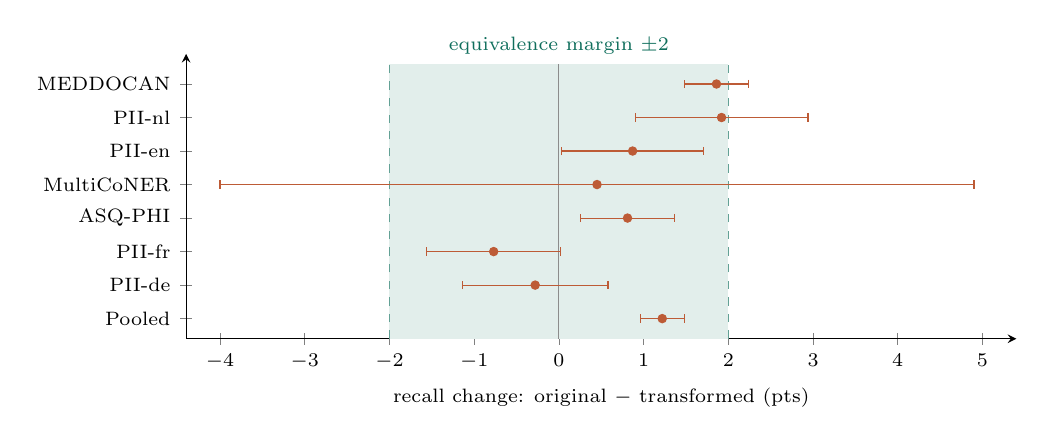
\begin{tikzpicture}
\begin{axis}[
  width=\linewidth, height=5.2cm,
  xmin=-4.4, xmax=5.4, xlabel={recall change: original $-$ transformed (pts)},
  xlabel style={font=\scriptsize}, tick label style={font=\scriptsize},
  ytick={1,2,3,4,5,6,7,8},
  yticklabels={Pooled,PII-de,PII-fr,ASQ-PHI,MultiCoNER,PII-en,PII-nl,MEDDOCAN},
  ymin=0.4, ymax=8.9, axis y line=left, axis x line=bottom, clip=false,
]
\fill[caccent!12] (axis cs:-2,0.4) rectangle (axis cs:2,8.6);
\draw[caccent!65,dashed] (axis cs:-2,0.4)--(axis cs:-2,8.6);
\draw[caccent!65,dashed] (axis cs:2,0.4)--(axis cs:2,8.6);
\draw[black!45] (axis cs:0,0.4)--(axis cs:0,8.6);
\addplot[only marks,mark=*,mark size=1.5pt,color=cclay,
  error bars/.cd,x dir=both,x explicit] coordinates {
  (1.22,1) +- (0.26,0.26) (-0.28,2) +- (0.86,0.86) (-0.77,3) +- (0.79,0.79)
  (0.81,4) +- (0.55,0.55) (0.45,5) +- (4.45,4.45) (0.87,6) +- (0.84,0.84)
  (1.92,7) +- (1.02,1.02) (1.86,8) +- (0.38,0.38)};
\node[font=\scriptsize,text=caccent,anchor=south] at (axis cs:0,8.6) {equivalence margin $\pm2$};
\end{axis}
\end{tikzpicture}
\caption{Per-benchmark equivalence (C3). Masked-span recall change (original~$-$~transformed) with 95\% CIs; the shaded band is the $\pm2$-pt equivalence margin. The pooled estimate and five of seven benchmarks sit fully inside; only MEDDOCAN and PII-nl reach past $+2$ (hence a $\pm3$ margin). MultiCoNER's wide interval reflects its 220 masked spans.}
\label{fig:forest}
\end{figure}

\begin{table}[t]\centering\small
\begin{adjustbox}{max width=\columnwidth}%
\begin{tabular}{lrrrl}
\toprule
Benchmark & Masked & O$\rightarrow$T & McN.\ $\chi^2$ & Margin\\
\midrule
ASQ-PHI & 5{,}427 & 91.9$\rightarrow$91.1 & 8.0 & $\pm2$\,\checkmark\\
MEDDOCAN & 31{,}978 & 73.4$\rightarrow$71.5 & 92.4 & $\pm3$\,\checkmark\\
MultiCoNER & 220 & 71.8$\rightarrow$71.4 & 0.0 & underpow.\\
PII en & 5{,}181 & 76.0$\rightarrow$75.1 & 4.0 & $\pm2$\,\checkmark\\
PII nl & 3{,}757 & 78.2$\rightarrow$76.3 & 13.1 & $\pm3$\,\checkmark\\
PII fr & 5{,}984 & 75.2$\rightarrow$75.9 & 3.5 & $\pm2$\,\checkmark\\
PII de & 4{,}565 & 76.3$\rightarrow$76.5 & 0.4 & $\pm2$\,\checkmark\\
\midrule
\textbf{Pooled} & \textbf{57{,}112} & \textbf{76.1$\rightarrow$74.9} & \textbf{82.1} & $\pm2$\,\checkmark\\
\bottomrule
\end{tabular}
\end{adjustbox}
\caption{Per-benchmark equivalence. O$\rightarrow$T = masked-span recall, original$\rightarrow$transform (\%). Pooled TOST $\Delta{=}2$: $p{=}3{\times}10^{-9}$.}\label{tab:c3}
\end{table}

\textbf{Redaction floor (C1).} We replace each masked value with \tp{*****}---destroying the surrogate signal---and re-detect with four detectors spanning all three families (Table~\ref{tab:c1}). The floor is sharply \emph{family-dependent}. Rule-based Presidio and the fine-tuned OBI tagger collapse to $\approx$0--4\% everywhere: they key on real surface tokens, so with the signal gone they recover almost nothing (the residual is spurious overlap on the \tp{*} run). Open LLMs behave differently---they partly \emph{recover} the masked span (Qwen-9B 6--58\%, Gemma-31B 13--80\%)---because a \tp{*****} run is itself a legible redaction cue a strong reader flags as ``something was here.'' This recovery is \emph{context-dependent}: highest on ASQ-PHI (short adversarial queries where one masked run dominates the prompt) and on the larger model, lowest on the dense multilingual PII sets. Even Gemma's floor stays far below its surrogate recall (Table~\ref{tab:c2}), so the conclusion holds across families---redaction destroys detectability that structure-preserving substitution keeps, and where a detector recovers anything from \tp{*****} it reads the mask, not the (absent) PHI.

\begin{table*}[t]\centering\small
\begin{adjustbox}{max width=\columnwidth}%
\begin{tabular}{lrrrrr}
\toprule
 & & \multicolumn{2}{c}{rule / fine-tuned} & \multicolumn{2}{c}{open LLM}\\
\cmidrule(lr){3-4}\cmidrule(lr){5-6}
Benchmark & \nk{N} & Presidio & OBI & Qwen-9B & Gemma-31B\\
\midrule
ASQ-PHI & \nk{267} & 0.0 & 0.7 & 58.1 & 79.8\\
MEDDOCAN & \nk{1{,}419} & 0.0 & 0.1 & 22.9 & 52.6\\
MultiCoNER & \nk{8} & -- & 0.0 & 25.0 & 12.5\\
PII en & \nk{210} & 1.9 & 1.0 & 10.0 & 37.6\\
PII nl & \nk{195} & 3.8 & 1.0 & 20.5 & 39.5\\
PII fr & \nk{220} & 2.2 & 0.5 & 5.9 & 38.2\\
PII de & \nk{204} & 0.0 & 1.0 & 11.8 & 41.7\\
\midrule
Mean & & \textbf{1.3} & \textbf{0.6} & 22.0 & 43.1\\
\bottomrule
\end{tabular}
\end{adjustbox}
\caption{C1 redaction floor: masked-span recall (\%) after replacing each masked value with \tp{*****}, across detector families. Rule/fine-tuned detectors collapse to $\approx$0; open LLMs partly recover the redaction cue (context-dependent). All floors sit well below the surrogate recall in Table~\ref{tab:c2}. \nk{N} (khaki) is the masked-span count in the 120-doc subsample shared by OBI, Qwen-9B and Gemma-31B; Presidio uses the full corpus (N${=}$531, 2{,}925, 471, 373, 544, 415 for its six rows). MultiCoNER contributes only 8 masked spans, so those cells are illustrative. Per-cell 95\% bootstrap CIs are reported in the extended (arXiv) version. Means are over each detector's benchmarks (Presidio: 6; others: 7).}\label{tab:c1}
\end{table*}

\textbf{Open-surrogate baseline (C2).} We replace the commercial generator with Faker on the same masked spans and re-score all four detectors (Table~\ref{tab:c2}); two findings hold \emph{across families}. \emph{Generality}: every detector retains high masked-span recall on the open surrogates---Presidio 78--98\%, OBI 64--100\%, Qwen-9B 77--100\%, Gemma-31B 83--100\% (family means 84--95\%)---so detectability preservation is a property of well-formed, same-type substitution, not of one vendor or one detector, and it reproduces without proprietary access. \emph{The residual is generator quality}: Faker, emitting clean canonical values, matches or exceeds the commercial transform precisely on the hard non-English benchmarks where the commercial surrogates truncate or garble (\S\ref{sec:error}); the stronger the detector, the smaller the residual (Gemma-31B mean 94.5\%).

\begin{table*}[t]\centering\small
\begin{adjustbox}{max width=\columnwidth}%
\begin{tabular}{lrrrrr}
\toprule
 & & \multicolumn{2}{c}{rule / fine-tuned} & \multicolumn{2}{c}{open LLM}\\
\cmidrule(lr){3-4}\cmidrule(lr){5-6}
Benchmark & \nk{N} & Presidio & OBI & Qwen-9B & Gemma-31B\\
\midrule
ASQ-PHI & \nk{267} & 97.7 & 100.0 & 100.0 & 100.0\\
MEDDOCAN & \nk{1{,}419} & 79.7 & 64.0 & 79.6 & 96.5\\
MultiCoNER & \nk{8} & -- & 100.0 & 87.5 & 100.0\\
PII en & \nk{210} & 89.2 & 89.5 & 76.7 & 90.0\\
PII nl & \nk{195} & 93.0 & 71.8 & 84.1 & 96.9\\
PII fr & \nk{220} & 78.5 & 79.5 & 81.4 & 83.2\\
PII de & \nk{204} & 78.1 & 84.8 & 77.9 & 95.1\\
\midrule
Mean & & 86.0 & 84.2 & 83.9 & \textbf{94.5}\\
\bottomrule
\end{tabular}
\end{adjustbox}
\caption{C2 open-surrogate (Faker) retention: masked-span recall (\%), across detector families. Every family stays high (means 84--95\%), so detectability preservation is generic to well-formed substitution, not tool- or detector-specific. \nk{N}, subsampling, and mean denominators as in Table~\ref{tab:c1}.}\label{tab:c2}
\end{table*}

\textbf{Leakage} barely moves ($+0.3$ to $+4.1$ pts across detectors; Table~\ref{tab:fullf1}), so surrogates are not systematically easier to miss than the PHI they replace.

\textbf{Where the loss lands (per benchmark).} Table~\ref{tab:perbench} breaks whole-document $\Delta$F1 out by benchmark and detector. The pattern is sharp: almost all of the loss concentrates on \textbf{ASQ-PHI}---short, sparse-PHI adversarial queries where a single substitution dominates the document score ($-0.09$ to $-0.18$)---while the other six benchmarks are essentially flat ($|\Delta\text{F1}|\le0.06$, most $\le0.03$). Even the fine-tuned OBI tagger and the rule-based Presidio move by at most a few thousandths on most benchmarks. This is the first sign that the effect tracks \emph{surrogate-generation difficulty} (short adversarial text, dense non-English identifiers) rather than detector family---made precise in the error analysis (\S\ref{sec:error}).


\textbf{What the transform does (examples).} Table~\ref{tab:examples} (appendix) shows the substitution qualitatively across languages and formats: each PHI value becomes a same-type surrogate while clinical shorthand, foreign-language syntax, and JSON structure are left byte-for-byte intact. On the well-formed English cases every surrogate is still detected across most of the panel.

\textbf{Coverage, reported separately.} All results above are measured \emph{on the spans the transform masks}. Coverage---how much true PHI it detects and replaces---is a distinct, detector-side axis. It tracks how closely a benchmark's annotation matches the transform's notion of sensitive content: it masks \textbf{80.9\%} of gold PHI on ASQ-PHI and \textbf{48.3\%} on MEDDOCAN, and less ($\approx$26\%) on general-domain NER/PII corpora whose annotated entities (encyclopedic names, generic places) fall outside that scope; a configuration sweep confirmed \tp{domain=General} maximizes coverage. A per-entity-type breakdown and a detection-vs-replacement diagnosis (the coverage gap is mostly a \emph{replacement}-step issue---$\approx$77\% of missed clinical identifiers were flagged by the transform's own detector but not substituted) are in Appendix~\ref{app:coverage}. Decoupling matters because the two failure modes have different owners and fixes: an under-masked span is a \emph{detection/replacement} miss, whereas a masked-but-missed surrogate is a \emph{generation} defect (§\ref{sec:error}). Conflating them on whole-document F1 (Table~\ref{tab:fullf1}) would let a high-coverage/low-quality transform and a low-coverage/high-quality one look identical. We therefore report coverage as context and reserve the utility claim for masked spans.

\textbf{Matching modes.} Unless noted, retention uses \emph{overlap} matching (detector flags any part of the surrogate span). Exact matching (Table~\ref{tab:ret}, left) additionally requires identical character boundaries and is therefore sensitive to surrogate length changes (``Anna~S.''$\rightarrow$``Maria~S.'' shifts the end offset); the $\sim$3-point exact$-$overlap gap is this boundary jitter, not missed PHI. Type matching (boundary~+~type) sits between the two and tracks overlap closely.

\section{Error Analysis}\label{sec:error}
\textbf{The lost population.} Pooled across detectors and masked spans: 40{,}165 (span$\times$detector) pairs found in both conditions; 3{,}300 lost. Half (50\%) of lost spans are the \emph{same length} as the original---so this is not a boundary effect. By type: LOCATION 27\%, NAME 23\%, DATE/AGE 22\%, ID/contact 19\%.

\textbf{Three failure modes---all generator-side.}
(1)~\emph{Malformed/truncated surrogates} (largest cause): \oldv{\tp{Chicago}}\arr\newv{\tp{Illino}}, \oldv{\tp{El~Paso}}\arr\newv{\tp{El}}, \oldv{\tp{Ciudad de la Habana}}\arr\newv{\tp{Cuidad de la Havana}}. The fragment no longer matches the lexical pattern detectors learned for real names/places; this is why span-level loss is highest on MEDDOCAN (6.9\%; Spanish, dense, identifier-heavy) and lowest on clean English ASQ-PHI (2.5\%).
(2)~\emph{Loss of salience}: a canonical entity replaced by an obscure one (\oldv{\tp{Cedars-Sinai}}\arr\newv{\tp{Vidant}}); detectors partly rely on pre-training familiarity, so swapping a famous value for a rare one removes the prior. Inherent to any value substitution; mainly costs weaker detectors.
(3)~\emph{\tp{x}-masking of IDs/emails}: \oldv{\tp{nachorutor@\dots}}\arr\newv{\tp{nxxxxxxxxx@\dots}}. The \tp{x} run preserves format but breaks the realistic-token pattern. This case is \emph{privacy-positive}---the original value is destroyed---even though it counts against recall.

\textbf{Quantifying the typology.} We classify a stratified 200-span sample (proportional across the seven benchmarks) by \emph{AI review}---an LLM labels each surrogate, with scripted \tp{x}-mask detection.\footnote{An AI review, \emph{not} human-validated; the released sheet records the labels, and human double-annotation is left to future work.} \textbf{77.0\%} of surrogates are well-formed, same-type values; of the 23\% with a defect, truncation/garbling dominates (12.5\%), then \tp{x}-masking (9.0\%), with salience loss rare (1.5\%); type-consistency is near-total (99.5\%). The \textbf{77\% well-formed rate tracks the 74.9\% masked-span recall}---detectors recover almost exactly the well-formed surrogates and miss the defective ones, so the residual is a surrogate-\emph{generation} problem, not a detection one.

\textbf{Implication.} Detectors are not getting worse at PHI; the small recall gap is driven by surrogate-generation quality (truncation, garbling, salience, \tp{x}-masking)---generating well-formed, in-distribution synthetic text is itself a hard problem~\citep{bao2024amr}. C2 confirms this: an open generator emitting clean canonical values matches or exceeds the commercial transform on exactly the hard non-English benchmarks where its surrogates truncate---so the residual tracks generator quality, not the act of substitution.

\section{Discussion}
\textbf{What the evidence supports.} Structure-preserving substitution does not hide well-formed PHI from downstream detection. Because the effect is equivalence-bounded within $\pm2$ points and ranking-preserving across a heterogeneous 11-detector panel, a transform of this quality can be inserted ahead of detection/analytics pipelines built for real clinical text without materially degrading downstream detection. \textbf{Generality (C2).} Faker preserves masked-span recall at least as well as the original across all six benchmarks, so $\pm2$ points appears to be a property of well-formed substitution rather than of one vendor; where the commercial generator trails, a cleaner generator closes the gap, locating the residual squarely in generation quality. \textbf{A reusable protocol.} The paired masked-span design and the TOST margin are not specific to one vendor or language---a template for auditing any structure-preserving privacy transform. \textbf{Deployment guidance.} A structure-preserving transform can be treated as admissible ahead of a detection/analytics pipeline when it clears a three-part check---detectability measured on masked spans only, the change inside an equivalence margin with ranking preserved, and surrogate outputs free of the three generator-side defects (truncation/garbling, salience loss, \tp{x}-masking) that drive the residual.

\section{Ethics and Data Statement}
All benchmarks are public or synthetic (ASQ-PHI synthetic; MEDDOCAN released for a shared task; PII-Masking-300k synthetic; MultiCoNER~v2 public). \textbf{No real patient data is used.} We release the 250-document subsets and scoring code with license notes. \textbf{Dual-use.} A utility-preserving de-identifier could in principle launder identifiable data into a fluent form; our masked-span/leakage reporting and the privacy-positive framing of \tp{x}-masking keep the privacy accounting explicit. \textbf{Conflict of interest.} The commercial transform evaluated as the case study is developed by a vendor with which one or more authors are affiliated (details withheld for anonymous review); the work was conducted with that vendor's support. To limit bias we (i)~frame the contribution as a reusable protocol, (ii)~include open-source baselines so results are reproducible without proprietary access, and (iii)~report leakage and coverage alongside utility.

\section{Limitations}
Coverage is reported but not the focus; a transform can preserve utility on what it masks while under-masking (the axes are independent by design). 250~docs/benchmark bounds per-benchmark power (though the pooled masked-span $N$ is large). C1/C2 span four detectors across families (Presidio full-corpus; OBI, Qwen-9B, Gemma-31B on a 120-doc/benchmark subsample); extending them to the full 11-detector panel is straightforward future work. LLM detectors are prompt-sensitive and their behaviour shifts with task framing and structural variation~\citep{gendron2024abstract,bao2024robustness}; we fix one prompt per model and release it with the code and data at the project's reproducibility page. Finally, all seven benchmarks are public or synthetic; validating the protocol on real-EHR corpora (n2c2, MIMIC-IV-Note, CARMEN-I) is future work pending the relevant data-use agreements.

\clearpage
\appendix

\section{Additional Results}\label{app:addl}
This appendix collects results referenced from the main text: the conservative whole-document view across all 11 detectors (Table~\ref{tab:fullf1}), the per-benchmark $\Delta$F1 breakdown (Table~\ref{tab:perbench}), the Presidio C1/C2 chart (Figure~\ref{fig:bars}), and worked transform examples (Table~\ref{tab:examples}).

\begin{figure}[htbp]
\centering
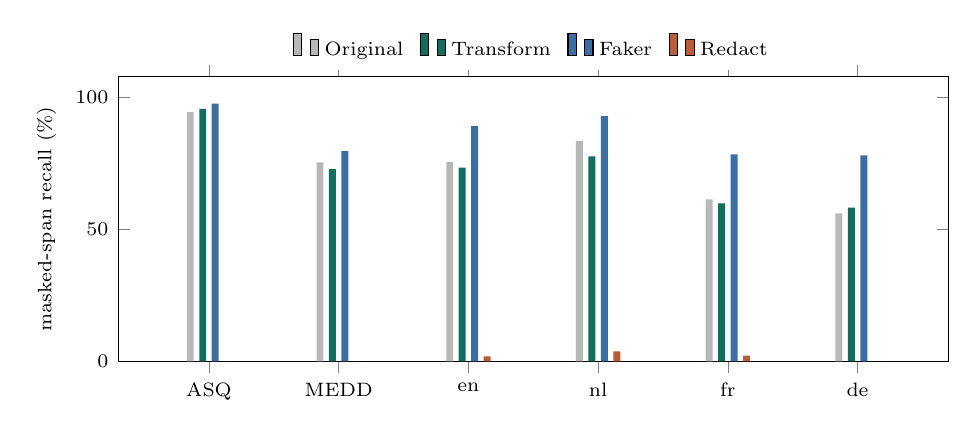
\begin{tikzpicture}
\begin{axis}[
  width=\linewidth, height=5.2cm, ybar, bar width=2.5pt,
  symbolic x coords={ASQ,MEDD,en,nl,fr,de}, xtick=data,
  ymin=0, ymax=108, ylabel={masked-span recall (\%)},
  ylabel style={font=\scriptsize}, tick label style={font=\scriptsize},
  legend style={font=\scriptsize,at={(0.5,1.02)},anchor=south,legend columns=4,draw=none,/tikz/every even column/.append style={column sep=4pt}},
  enlarge x limits=0.14,
]
\addplot[fill=black!28,draw=none] coordinates {(ASQ,94.5)(MEDD,75.4)(en,75.6)(nl,83.6)(fr,61.4)(de,56.1)};
\addplot[fill=caccent,draw=none] coordinates {(ASQ,95.7)(MEDD,72.9)(en,73.5)(nl,77.7)(fr,59.9)(de,58.3)};
\addplot[fill=cblue,draw=none] coordinates {(ASQ,97.7)(MEDD,79.7)(en,89.2)(nl,93.0)(fr,78.5)(de,78.1)};
\addplot[fill=cclay,draw=none] coordinates {(ASQ,0)(MEDD,0)(en,1.9)(nl,3.8)(fr,2.2)(de,0)};
\legend{Original,Transform,Faker,Redact}
\end{axis}
\end{tikzpicture}
\caption{What structure preservation buys, shown for Presidio (full original/transform/Faker/redact columns). Transform tracks the original, the open Faker baseline is at least as high, and redaction collapses to $\approx$0. The family-dependent floor and open-surrogate retention across four detectors are in Tables~\ref{tab:c1}--\ref{tab:c2}.}
\label{fig:bars}
\end{figure}

\begin{table*}[tbp]\centering\small
\begin{tabular}{p{2.3cm}p{6.0cm}p{6.0cm}}
\toprule
Case & Original & Transformed\\
\midrule
ASQ-PHI (clinical query) & \dots a \oldv{34}-year-old female \dots like \oldv{Anna~S.}, \dots at Methodist Hospital on \oldv{April~12,~2023}? & \dots a \newv{35}-year-old female \dots like \newv{Maria~S.}, \dots at Methodist Hospital on \newv{March~13,~2021}?\\
\addlinespace
ASQ-PHI (shorthand) & Rec mgmt of \oldv{70yo} M w/ CHF, seen by Dr.~\oldv{John~L.} at \oldv{Mt.~Sinai} on \oldv{Feb~21,~2023}. alt tx options\dots & Rec mgmt of \newv{73yo} M w/ CHF, seen by Dr.~\newv{James~L.} at \newv{Mt.~Egypt} on \newv{Nov~19,~2021}. alt tx options\dots\\
\addlinespace
PII (German) & \dots erm\"achtigen hiermit \oldv{Monsignore}, \dots Mit Datum \oldv{23/07/2011}\dots & \dots erm\"achtigen hiermit \newv{Fulgenzio}, \dots Mit Datum \newv{24/07/2011}\dots\\
\addlinespace
PII (French, JSON) & \tp{\{"Date":"\oldv{20/05/2022}", "City":"Saint-Priest", "Username":"phprosdocimo"\}} & \tp{\{"Date":"\newv{21/05/2023}", "City":"Saint-Priest", "Username":"phprosdocimo"\}}\\
\bottomrule
\end{tabular}
\caption{Worked transform examples. Only the sensitive value moves; abbreviations (\tp{w/ CHF}, \tp{alt tx}), non-English syntax, and JSON keys/quotes/indentation are preserved, so downstream parsers and detectors keep working. In the JSON case the transform changes only the date value and leaves the (also-sensitive-looking) username untouched---a coverage decision, not a utility one (see below).}\label{tab:examples}
\end{table*}

\begin{table}[htbp]\centering\small
\begin{adjustbox}{max width=\columnwidth}%
\begin{tabular}{lrrrrr}
\toprule
Detector & \multicolumn{2}{c}{F1} & $\Delta$ & \multicolumn{2}{c}{Leak}\\
\cmidrule(lr){2-3}\cmidrule(lr){5-6}
 & orig & transf & F1 & orig & transf\\
\midrule
Gemma 4 31B & .755 & .710 & $-.045$ & .255 & .285\\
Gemma 4 E4B & .737 & .698 & $-.038$ & .276 & .311\\
Llama 3.3-70B & .725 & .728 & $+.003$ & .245 & .262\\
Qwen 3.5-35B-A3B & .715 & .668 & $-.047$ & .254 & .295\\
OpenAI GPT-5 & .705 & .674 & $-.032$ & .308 & .333\\
Qwen 3.5-9B & .655 & .621 & $-.034$ & .391 & .422\\
Qwen 3.5-4B & .567 & .533 & $-.034$ & .483 & .515\\
Presidio & .416 & .398 & $-.018$ & .553 & .570\\
DeepSeek V2-Lite & .409 & .384 & $-.025$ & .672 & .696\\
Llama 3.1-8B & .391 & .376 & $-.015$ & .633 & .650\\
OBI \tp{deid\_roberta} & .041 & .040 & $-.002$ & .941 & .944\\
\bottomrule
\end{tabular}
\end{adjustbox}
\caption{Whole-document view (all 11 detectors), mean over 7 benchmarks. Span-level F1 (type match) and leakage ($1-$recall). Conservative: it includes untouched spans and boundary penalties. Ranking is preserved and $\Delta$F1 is bounded.}\label{tab:fullf1}
\end{table}

\begin{table*}[tbp]\centering\small
\begin{tabular}{lrrrrrrr}
\toprule
Detector & ASQ-PHI & MEDDOCAN & PII en & PII nl & PII fr & PII de & MultiCoNER\\
\midrule
Gemma 4 31B & $-.175$ & $-.017$ & $-.043$ & $-.038$ & $-.014$ & $-.016$ & $-.009$\\
Gemma 4 E4B & $-.106$ & $-.060$ & $-.032$ & $-.021$ & $-.018$ & $-.025$ & $-.007$\\
Qwen 3.5-35B-A3B & $-.132$ & $-.034$ & $-.026$ & $-.034$ & $-.040$ & $-.054$ & $-.007$\\
OpenAI GPT-5 & $-.098$ & $-.046$ & $-.049$ & $-.019$ & $+.008$ & $-.005$ & $-.014$\\
Qwen 3.5-9B & $-.123$ & $-.017$ & $-.025$ & $-.010$ & $-.034$ & $-.024$ & $-.008$\\
Qwen 3.5-4B & $-.086$ & $-.055$ & $-.034$ & $-.028$ & $-.015$ & $-.023$ & $+.002$\\
Presidio & $+.003$ & $-.037$ & $-.032$ & $-.015$ & $-.020$ & $-.015$ & $-.007$\\
Llama 3.1-8B & $-.108$ & $+.023$ & $-.014$ & $+.007$ & $-.009$ & $+.003$ & $-.006$\\
OBI \tp{deid\_roberta} & $+.001$ & $-.008$ & $-.004$ & $-.001$ & $+.003$ & $-.002$ & $-.001$\\
\bottomrule
\end{tabular}
\caption{Per-benchmark whole-document $\Delta$F1 (transformed $-$ original; negative = drop). Almost all loss lands on ASQ-PHI; the other six benchmarks are flat. Llama~3.3-70B and DeepSeek~V2-Lite omitted for space (both flat; see Table~\ref{tab:fullf1} for their pooled $\Delta$F1).}\label{tab:perbench}
\end{table*}


\section{Coverage Details}\label{app:coverage}
Coverage (\S\ref{sec:results}) is the fraction of a benchmark's gold PHI whose characters the transform actually changed (difflib alignment). Table~\ref{tab:covtype} breaks it down by entity type on the clinical sets (ASQ-PHI~+~MEDDOCAN). High-frequency free-text types (names, dates) are masked well; the weak spots are high-sensitivity structured identifiers and geography---exactly the HIPAA Safe Harbor items that most need masking.

\begin{table}[h]\centering\small
\begin{adjustbox}{max width=\columnwidth}%
\begin{tabular}{lr}
\toprule
Entity type (clinical) & Coverage\\
\midrule
NAME / person & 75.0\%\\
DATE / age & 73.4\%\\
ID / contact (MRN, patient ID, phone, email) & 50.7\%\\
ORG / facility & 46.6\%\\
LOCATION / address & 43.7\%\\
\bottomrule
\end{tabular}
\end{adjustbox}
\caption{Coverage by entity type on clinical benchmarks. Overall the transform altered 39\% of annotated PII (54\% on clinical sets); general-domain corpora sit near 26\%.}\label{tab:covtype}
\end{table}

\textbf{Detection vs.\ replacement.} On a sample of 8 MEDDOCAN documents (62 missed ID/location spans), $48/62$ ($\approx$77\%) of the \emph{un}masked identifiers were nonetheless flagged as sensitive by the transform's own detector---they were detected but not substituted; only $14/62$ (23\%) were undetected. The coverage gap is therefore mostly a \emph{replacement-step} issue (act on everything the detector surfaces), which is more tractable than raising detection recall. (Small sample; ``detected'' judged by loose token overlap, so 77\% is directional.) Concrete unmasked HIPAA identifiers included patient IDs (\tp{80926}, \tp{7845693}), care-contact IDs (\tp{4387684}), and facilities/geography (\tp{Hospital de Cruces}, \tp{Espa\~na}, postal codes \tp{41005}, \tp{28047}).

\section{Representative Per-Detector Examples}\label{app:examples}

\textbf{All-detector overlay on one document (``ranking proof'').} All eleven detectors' predictions on one transformed document (\tp{asq\_00001}), overlaid on the text and sorted by this document's F1: \hg{green}~=~correctly caught PHI, \hy{yellow}~=~false positive, \hr{red}~=~missed PHI (leakage). The four gold surrogate values are \tp{John T.}, the \emph{x}-masked location \tp{Saint. Vxxxxxxxx}, \tp{April 25th, 2018}, and the ID \tp{987654321}. Eight of eleven detectors tag all four cleanly (F1~100); the two floor detectors, Presidio and DeepSeek, miss the \emph{x}-masked location surrogate (§\ref{sec:error} mode~3)---DeepSeek also drops the numeric ID---and OBI over-fragments boundaries and false-fires on the age \tp{60}. The surrogate values shown are the transform's output, not the original PHI.

{\footnotesize
\setlength{\fboxsep}{1pt}%
\newcommand{\panel}[3]{\par\vspace{2.5pt}\noindent\fcolorbox{cline}{white}{\parbox{0.965\linewidth}{%
\textbf{#1}\hfill{\scriptsize\color{cmuted}#2}\\[2pt]\ttfamily\scriptsize #3}}}
\panel{Gold (reference)}{4 PHI spans}{Evaluation of long-term outcomes for bypass surgery in patients over 60, referencing Mr. \hg{John T.}, operated at \hg{Saint. Vxxxxxxxx} on \hg{April 25th, 2018} (ID: \hg{987654321})?}
\panel{OpenAI GPT-5}{tp 4 $\cdot$ fp 0 $\cdot$ missed 0 $\cdot$ F1 100\%}{Evaluation of long-term outcomes for bypass surgery in patients over 60, referencing \hg{Mr. John T.}, operated at \hg{Saint. Vxxxxxxxx} on \hg{April 25th, 2018} (\hg{ID: 987654321})?}
\panel{Llama 3.1-8B}{tp 4 $\cdot$ fp 0 $\cdot$ missed 0 $\cdot$ F1 100\%}{Evaluation of long-term outcomes for bypass surgery in patients over 60, referencing Mr. \hg{John T.}, operated at \hg{Saint. Vxxxxxxxx} on \hg{April 25th, 2018} (ID: \hg{987654321})?}
\panel{Qwen 3.5-4B}{tp 4 $\cdot$ fp 0 $\cdot$ missed 0 $\cdot$ F1 100\%}{Evaluation of long-term outcomes for bypass surgery in patients over 60, referencing \hg{Mr. John T.}, operated at \hg{Saint. Vxxxxxxxx} on \hg{April 25th, 2018} (ID: \hg{987654321})?}
\panel{Gemma 4 31B}{tp 4 $\cdot$ fp 0 $\cdot$ missed 0 $\cdot$ F1 100\%}{Evaluation of long-term outcomes for bypass surgery in patients over 60, referencing \hg{Mr. John T.}, operated at \hg{Saint. Vxxxxxxxx} on \hg{April 25th, 2018} (ID: \hg{987654321})?}
\panel{Llama 3.3-70B}{tp 4 $\cdot$ fp 0 $\cdot$ missed 0 $\cdot$ F1 100\%}{Evaluation of long-term outcomes for bypass surgery in patients over 60, referencing Mr. \hg{John T.}, operated at \hg{Saint. Vxxxxxxxx} on \hg{April 25th, 2018} (ID: \hg{987654321})?}
\panel{Qwen 3.5-35B-A3B}{tp 4 $\cdot$ fp 0 $\cdot$ missed 0 $\cdot$ F1 100\%}{Evaluation of long-term outcomes for bypass surgery in patients over 60, referencing \hg{Mr. John T.}, operated at \hg{Saint.} \hg{Vxxxxxxx}x on \hg{April 25th}, \hg{2018} (ID: \hg{987654321})?}
\panel{Gemma 4 E4B}{tp 4 $\cdot$ fp 0 $\cdot$ missed 0 $\cdot$ F1 100\%}{Evaluation of long-term outcomes for bypass surgery in patients over 60, referencing Mr. \hg{John T.}, operated at \hg{Saint. Vxxxxxxxx} on \hg{April 25th, 2018} (ID: \hg{987654321})?}
\panel{Qwen 3.5-9B}{tp 4 $\cdot$ fp 0 $\cdot$ missed 0 $\cdot$ F1 100\%}{Evaluation of long-term outcomes for bypass surgery in patients over 60, referencing \hg{Mr. John T.}, operated at \hg{Saint. Vxxxxxxxx} on \hg{April 25th, 2018} (ID: \hg{987654321})?}
\panel{OBI deid\_roberta}{tp 4 $\cdot$ fp 1 $\cdot$ missed 0 $\cdot$ F1 89\%}{Evaluation of long-term outcomes for bypass surgery in patients over \hy{60}, referencing Mr. \hg{John} \hg{T}., operated at \hg{Saint}. \hg{Vxxxxxxxx} on \hg{April 25th,} \hg{2018} (ID: \hg{987654321})?}
\panel{Microsoft Presidio}{tp 3 $\cdot$ fp 1 $\cdot$ missed 1 $\cdot$ F1 75\%}{Evaluation of long-term outcomes for bypass surgery in patients over \hy{60}, referencing Mr. \hg{John T.}, operated at \hr{Saint. Vxxxxxxxx} on \hg{April 25th, 2018} (ID: \hg{987654321})?}
\panel{DeepSeek V2-Lite}{tp 2 $\cdot$ fp 0 $\cdot$ missed 2 $\cdot$ F1 67\%}{Evaluation of long-term outcomes for bypass surgery in patients over 60, referencing Mr. \hg{John T.}, operated at \hr{Saint. Vxxxxxxxx} on \hg{April 25th, 2018} (ID: \hr{987654321})?}

\par}
\vspace{4pt}

\textbf{A harder case: a dense Spanish clinical header.} Figure-style overlay on a 260-character window of a MEDDOCAN document (\tp{S0210-\dots008-1}), where the same eleven detectors diverge far more---F1 from 96 down to 0. On dense, identifier-heavy non-English text the \emph{per-document} ranking reshuffles (here DeepSeek and Qwen-4B lead, while Llama~3.1-8B finds nothing in this window), even though the \emph{aggregate} ranking over 250 documents is stable (Table~\ref{tab:fullf1}). The garbled surrogate \tp{Cuidad Real} (from \tp{Ciudad Real}) is still caught by most detectors; the misses cluster on the professional-licence ID \tp{03 14 16485}, the sex fields, and the repeated age---the identifier types with the weakest coverage and the hardest surrogates (Appendix~\ref{app:coverage}).

{\footnotesize
\setlength{\fboxsep}{1pt}%
\newcommand{\panel}[3]{\par\vspace{2.5pt}\noindent\fcolorbox{cline}{white}{\parbox{0.965\linewidth}{%
\textbf{#1}\hfill{\scriptsize\color{cmuted}#2}\\[2pt]\ttfamily\scriptsize #3}}}
\panel{Gold (reference)}{12 PHI spans}{\hg{Cuidad Real}. CP: \hg{13002}. Datos asistenciales. Referencia de nacimiento: \hg{24/10/1963}. País: \hg{España}. Mejores: \hg{53 años} Sexo: \hg{H}. Referencia de Ingreso: \hg{14/12/2017}. Episodio: \hg{746589123}. Médico: \hg{Luis Ruiz Camuñas} N\textordmasculine Col: \hg{03 14 16485}. Historia Actual: \hg{Varón} de \hg{53 años} q}
\panel{DeepSeek V2-Lite}{tp 11 $\cdot$ fp 0 $\cdot$ missed 1 $\cdot$ F1 96\%}{\hg{Cuidad Real}. CP: \hg{13002}. Datos asistenciales. Referencia de nacimiento: \hg{24/10/1963}. País: \hg{España}. Mejores: \hg{53 años} Sexo: \hg{H}. Referencia de Ingreso: \hg{14/12/2017}. Episodio: \hg{746589123}. Médico: \hg{Luis Ruiz Camuñas} N\textordmasculine Col: \hr{03 14 16485}. Historia Actual: \hg{Varón de 53 años q}}
\panel{Qwen 3.5-4B}{tp 11 $\cdot$ fp 0 $\cdot$ missed 1 $\cdot$ F1 96\%}{\hg{Cuidad Real.} CP: \hg{13002.} Datos asistenciales. Referencia de nacimiento: \hg{24/10/1963.} País: \hg{España.} Mejores: \hg{53} años Sexo: \hg{H.} Referencia de Ingreso: \hg{14/12/2017.} Episodio: \hg{746589123.} Médico: \hg{Luis Ruiz Camuñas} N\textordmasculine Col: \hg{03} 14 \hg{16485.} Historia Actual: \hr{Varón} de \hg{53} años q}
\panel{OBI deid\_roberta}{tp 10 $\cdot$ fp 0 $\cdot$ missed 2 $\cdot$ F1 91\%}{\hg{Cu}idad \hg{Real}. CP: \hg{13}002. Datos asistenciales. Referencia de nacimiento: \hg{24/10/1963}. País: \hg{Esp}aña. Mejores: \hg{53} años Sexo: \hr{H}. Referencia de Ingreso: \hg{14/12/2017}. Episodio: \hg{746589123}. Médico: \hg{Luis Ruiz} \hg{Camuñ}as N\textordmasculine Col: \hg{03 14} \hg{16485}. Historia Actual: \hr{Varón} de \hg{53} años q}
\panel{Qwen 3.5-9B}{tp 10 $\cdot$ fp 0 $\cdot$ missed 2 $\cdot$ F1 91\%}{\hg{Cuidad Real}. CP: \hg{13002}. Datos asistenciales. Referencia de nacimiento: \hg{24/10/1963}. País: \hg{España}. Mejores: \hg{53} años Sexo: \hr{H}. Referencia de Ingreso: \hg{14/12/2017}. Episodio: \hg{746589123}. Médico: \hg{Luis Ruiz Camuñas} N\textordmasculine Col: \hg{03 14 16485}. Historia Actual: \hr{Varón} de \hg{53} años q}
\panel{Gemma 4 31B}{tp 9 $\cdot$ fp 0 $\cdot$ missed 3 $\cdot$ F1 86\%}{\hg{Cuidad Real}. CP: \hg{13002}. Datos asistenciales. Referencia de nacimiento: \hg{24/10/1963}. País: \hr{España}. Mejores: \hg{53 años} Sexo: \hr{H}. Referencia de Ingreso: \hg{14/12/2017}. Episodio: \hg{746589123}. Médico: \hg{Luis Ruiz Camuñas} N\textordmasculine Col: \hg{03 14 16485}. Historia Actual: \hr{Varón} de \hg{53 años} q}
\panel{Qwen 3.5-35B-A3B}{tp 9 $\cdot$ fp 1 $\cdot$ missed 3 $\cdot$ F1 82\%}{\hg{Cuidad Real}. CP: \hg{13002}. Datos asistenciales. Referencia de nacimiento: \hg{24/10/1963}. País: \hg{España}. Mejores: \hg{53} años Sexo: \hr{H}. Referencia de Ingreso: \hg{14/12/2017}. Episodio: \hg{746589123}. Médico: \hg{Luis Ruiz Camuñas} \hy{N\textordmasculine }Col: \hg{03 14 16485}. Historia Actual: \hr{Varón} de \hr{53 años} q}
\panel{OpenAI GPT-5}{tp 8 $\cdot$ fp 0 $\cdot$ missed 4 $\cdot$ F1 80\%}{\hg{Cuidad Real}. CP: \hg{13002}. Datos asistenciales. Referencia de nacimiento: \hg{24/10/1963}. País: \hr{España}. Mejores: \hg{53} años Sexo: \hr{H}. Referencia de Ingreso: \hg{14/12/2017}. Episodio: \hg{746589123}. Médico: \hg{Luis Ruiz Camuñas} N\textordmasculine Col: \hg{03 14 16485}. Historia Actual: \hr{Varón} de \hr{53 años} q}
\panel{Llama 3.3-70B}{tp 8 $\cdot$ fp 0 $\cdot$ missed 4 $\cdot$ F1 80\%}{\hg{Cuidad Real}. CP: \hg{13002}. Datos asistenciales. Referencia de nacimiento: \hg{24/10/1963}. País: \hr{España}. Mejores: \hg{53} años Sexo: \hr{H}. Referencia de Ingreso: \hg{14/12/2017}. Episodio: \hg{746589123}. Médico: \hg{Luis Ruiz Camuñas} N\textordmasculine Col: \hg{03 14 16485}. Historia Actual: \hr{Varón} de \hr{53 años} q}
\panel{Gemma 4 E4B}{tp 8 $\cdot$ fp 0 $\cdot$ missed 4 $\cdot$ F1 80\%}{\hg{Cuidad Real}. CP: \hg{13002}. Datos asistenciales. Referencia de nacimiento: \hg{24/10/1963}. País: \hr{España}. Mejores: \hg{53} años Sexo: \hr{H}. Referencia de Ingreso: \hg{14/12/2017}. Episodio: \hr{746589123}. Médico: \hg{Luis Ruiz Camuñas} N\textordmasculine Col: 03 14 1\hg{6}485. Historia Actual: \hr{Varón} de \hg{53} años q}
\panel{Microsoft Presidio}{tp 6 $\cdot$ fp 1 $\cdot$ missed 6 $\cdot$ F1 63\%}{\hg{Cuidad Real}. CP: \hr{13002}. Datos asistenciales. Referencia de nacimiento: \hg{24/10/1963}. \hy{País}: \hg{España}. Mejores: \hr{53 años} Sexo: \hr{H}. Referencia de Ingreso: \hg{14/12/2017}. Episodio: \hr{746589123}. Médico: \hg{Luis Ruiz Camuñas N\textordmasculine Col}: \hg{03 14 16485}. Historia Actual: \hr{Varón} de \hr{53 años} q}
\panel{Llama 3.1-8B}{tp 0 $\cdot$ fp 0 $\cdot$ missed 12 $\cdot$ F1 0\%}{\hr{Cuidad Real}. CP: \hr{13002}. Datos asistenciales. Referencia de nacimiento: \hr{24/10/1963}. País: \hr{España}. Mejores: \hr{53 años} Sexo: \hr{H}. Referencia de Ingreso: \hr{14/12/2017}. Episodio: \hr{746589123}. Médico: \hr{Luis Ruiz Camuñas} N\textordmasculine Col: \hr{03 14 16485}. Historia Actual: \hr{Varón} de \hr{53 años} q}

\par}
\vspace{4pt}

\textbf{Agreement on well-formed surrogates.} On clean English (ASQ-PHI), a plausible same-type surrogate is caught by nearly the whole panel (Table~\ref{tab:agree}): the substitution is invisible to detection. Divergence is confined to the two floor detectors (Llama~3.1-8B, DeepSeek~V2-Lite).

\begin{table}[h]\centering\small
\begin{adjustbox}{max width=\columnwidth}%
\begin{tabular}{llr}
\toprule
Document & Surrogate span (type) & Caught\\
\midrule
asq\_00000 & Maria S.\ (NAME) & 10/11\\
asq\_00000 & Methodist Hospital (LOC) & 9/11\\
asq\_00000 & March 13, 2021 (DATE) & 9/11\\
asq\_00003 & James L.\ (NAME) & 11/11\\
asq\_00003 & Mt.\ Egypt (LOC) & 11/11\\
asq\_00003 & Nov 19, 2021 (DATE) & 11/11\\
\bottomrule
\end{tabular}
\end{adjustbox}
\caption{Number of detectors (of 11) that find each well-formed surrogate. Same-type swaps stay broadly detectable.}\label{tab:agree}
\end{table}

\textbf{Representative losses, by failure type.} Table~\ref{tab:lost} shows genuine ``lost'' cases (MEDDOCAN): the original value was found by most detectors, but a defective surrogate is found by few. Each maps to one of the three failure types in \S\ref{sec:error}, and the drop is shared across the panel---i.e.\ it is a property of the surrogate, not of any one detector.

\begin{table}[h]\centering\small
\begin{adjustbox}{max width=\columnwidth}%
\begin{tabular}{p{3.5cm}rl}
\toprule
Original $\rightarrow$ surrogate & O\,$\rightarrow$\,T & Type\\
\midrule
\oldv{\tp{Cuba}}\arr\newv{\tp{Havana}} & 9\,$\rightarrow$\,2 & salience\\
\oldv{\tp{San Fernando}}\arr\newv{\tp{Francsico Luis}} & 8\,$\rightarrow$\,3 & garbled\\
\oldv{\tp{C\'adiz}}\arr\newv{\tp{Cadiz}} & 8\,$\rightarrow$\,4 & accent stripped\\
\oldv{\tp{Cecilio Pujaz\'on}}\arr\newv{\tp{ Pujaz\'on}} & 8\,$\rightarrow$\,4 & truncation\\
\oldv{\tp{ignaciotorne@\dots}}\arr\newv{\tp{ixxxxxxxxxxx@\dots}} & 9\,$\rightarrow$\,2 & \tp{x}-mask\\
\oldv{\tp{23/07/1948}}\arr\newv{\tp{2xxxxxxxx}} & 11\,$\rightarrow$\,4 & \tp{x}-mask\\
\oldv{\tp{40}}\arr\newv{\tp{35}} (age) & 9\,$\rightarrow$\,2 & bare number\\
\bottomrule
\end{tabular}
\end{adjustbox}
\caption{Representative lost spans on MEDDOCAN. O\,$\rightarrow$\,T = detectors finding the original vs.\ the surrogate (panel of 11--12; original includes one extra decoding variant). Losses are shared across detectors and align with the \S\ref{sec:error} typology.}\label{tab:lost}
\end{table}


\bibliography{refs}
\end{document}
